\documentclass[11pt]{article}

\usepackage[english]{babel}
\usepackage{csquotes}
\usepackage{amsmath}
\usepackage{amssymb}
\usepackage{chngcntr}

\usepackage{graphicx}
\graphicspath{{../img}}

\usepackage{hyperref}
\usepackage{bm}
\usepackage[final,expansion=alltext]{microtype}
\usepackage{blindtext}
% \usepackage{enumitem}

\usepackage[style=numeric]{biblatex}
\bibliography{references.bib}

% geometry of the page

\usepackage[top=1in, bottom=1in, left=1in, right=1in]{geometry}

% paragraph spacing

\title{Intermediate Report: Multi-Fidelity Bayesian Optimization for Wind Farm Layout Optimization}
\author{Aman Choudhri (\texttt{ac4972})}
\date{\today}


\begin{document}

\maketitle

\section{Methods}

\subsection{Problem Setup}
Let $X \in \mathbb{R}^{N \times 2}$ represent the locations of $N$ wind turbines. 
For a given incoming wind speed $v$ at direction $\phi$, write the power produced
by the farm (as estimated by a large eddy simulation) as $f_\text{LES}(X, v, \phi)$

Our ultimate objective of interest is the expected power production of a wind farm
over a historical wind condition distribution $p(v, \phi)$. We write this objective as
\[
    g_p(X) := \mathbb{E}_{p(v, \phi)} [f_\text{LES}(X, v, \phi)]
.\] 

% Our problem of interest then, is
% \begin{align*}
%     \text{maximize}_{X}& \quad g_p(X) \\
%     \text{subject to}& \quad ||x_i - x_j|| > C \quad \forall i,j \in \{1,\ldots,N\}, i \neq j \\
%     & \quad x_i \in \Omega \quad \forall i \in \{1,\ldots,N\}
% \end{align*}
%
Denote our analytic approximation to the ``true'' power production
$f_\text{LES}$ by $f_\text{approx}$. Our goal is to solve the above
optimization problem given a fixed evaluation budget, where we assume fixed
evaluation costs for each fidelity, $c_\text{LES}$ and $c_\text{approx}$.

To simplify the computation for this paper, we fix one incoming wind condition $v, \phi$,
solving:
\begin{align*}
    \text{maximize}_{X}& \quad f_\text{LES}(X, v, \phi) \\
    \text{subject to}& \quad x_i \in \Omega \quad \forall i \in \{1,\ldots,N\}
                     % & \quad ||x_i - x_j|| > C \quad \forall i,j \in \{1,\ldots,N\}, i \neq j \\
\end{align*}
% where $C$ represents the minimum allowable spacing between turbines (typically
% a multiple of the turbine rotor diameter) and $\Omega$ represents the available land
% area for the wind farm.
where $\Omega$ represents the available land area for the wind farm.

% \subsection{Analytic Wake Model}
% There are a variety of analytical wake models, based on various approximations
% and kinematic assumptions. See
% \cite{mudafortComparisonSteadystateAnalytical2024} for a recent survey of the
% field. Following \cite{bempedelisDatadrivenOptimisationWind2024} and
% \cite{moleMultiFidelityBayesianOptimisation2024}, we'll use the Gauss-curl
% hybrid (GCH) model \cite{niayifarAnalyticalModelingWind2016}.  The GCH model
% represents wind turbine wakes using Gaussian-shaped velocity deficits that
% spread downstream, with additional modeling terms for the rotational motion of
% the flow.
%
% We use the open source GCH implementation from the \texttt{FLORIS} Python package
% \cite{mudafortNRELFlorisV4212024}.
%
% \subsection{Computational Fluid Dynamics Simulation}
% Direct numerical solutions to the Navier-Stokes equations are computationally
% infeasible due to the large length scale range of the turbulent structures
% in and around wind farms \cite{bretonSurveyModellingMethods2017}. Large eddy simulations
% have emerged as a popular approximation scheme, balancing concerns of accuracy and efficiency.
% See \cite{mehtaLargeEddySimulation2014} for a full review.
%
% In this paper, again following \cite{bempedelisDatadrivenOptimisationWind2024,
% moleMultiFidelityBayesianOptimisation2024}, we use the \texttt{WInc3D} large
% eddy simulation solver framework \cite{deskosWInc3DNovelFramework2020}.
% Turbines are represented using the non-rotational actuator disk model (ADM-NR)
% approximation \cite{meyersLargeEddySimulations2010}, an approximation
% scheme that represents wind turbines as a solid porous disk through which wind flows, removing
% the need to model the effects of specific turbine blades. The ADM-NR model is commonly used
% in practice due to its accuracy and efficiency \cite{revazLargeEddySimulationWind2021} compared to
% other modeling choices like the actuator line model. See \cite{bretonSurveyModellingMethods2017} for
% a more detailed survey of rotor modeling methods.

\subsection{Optimization Approach}
\label{sec:opt_approach}

In this work, we follow the multi-task BO (MTBO) approach introduced in
\cite{swerskyMultiTaskBayesianOptimization2013} and shown in \cite{lethamBayesianOptimizationPolicy2019}
to be successful for regimes where one observation model is
significantly more expensive to evaluate.

Specifically, the different evaluation modes, $f_\text{approx}$ and
$f_\text{LES}$ are modeled using the intrinsic model of coregionalization (ICM).
Specifically, it posits two underlying independent Gaussian processes,
\[
    h_{1}, h_{2} \sim_{\text{iid}} \mathcal{GP}(0, \kappa)
,\]
that are linearly mixed to yield the observation modes as
\begin{align*}
    f_\text{approx} &= a^{(1)}_\text{approx} h_1 + a^{(2)}_\text{approx} h_{2} \\
    f_\text{LES} &= a^{(1)}_\text{LES} h_1 + a^{(2)}_\text{LES} h_{2}
.\end{align*}

The mixing coefficients $a$ are learned by maximizing marginal log
likelihood along with kernel hyperparameters. In this paper, we use the ARD Matern kernel with
smoothness $\nu = 5 / 2$.

The acquisition function for this model is noiseless batch expected improvement
(qEI), with incumbents defined over LES observations only. For a batch size of
$B$, this is given by
\[
    \alpha (X | D_\text{LES}, D_\text{GCH}) = \mathbb{E} \left[
        \max_{i = 1, \ldots , B} \max\left(0, f_\text{LES}(X_i) - f_\text{LES}^* \right) \ \big| \
        D_\text{LES} \cup D_\text{GCH}
    \right]
,\] 
for incumbent $f^*_\text{LES}$ defined as $\max_{x \in D_\text{LES}}
f_\text{LES}(x)$. To simplify the implementation, the reference paper
\cite{lethamBayesianOptimizationPolicy2019} alternates using this acquisition function
to pick batches for the cheap and expensive observation models, with different batch sizes for each.
We follow this design, trading off batches evaluated using GCH and LES.

We do make one notable change relative to the MTBO paper: namely, we acquire
and observe the cheap evaluations within a ``batch'' sequentially. This does incur
a cost overhead for more acquisition function maximizations. The hope was that
the expensive LES computation would dominate the optimization procedure runtime,
meaning this extra acquisition overhead would be negligible and yield essentially free
performance improvement.

\section{Results}
We optimized the placement of only $N = 4$ turbines as a proof of concept (by
comparison, the authors of \cite{bempedelisDatadrivenOptimisationWind2024}
picked $N = 16$) This limits the difficulty of the optimization problem and
the cost of running large eddy simulations, but include enough turbines that
wake effects would be non-negligible.

For our turbines, we employed the commonly-used \texttt{NREL-5MW}
\cite{jonkmanDefinition5MWReference2009} reference turbine specification. The
turbines have a diameter of $D =  126m$ and a hub height of $90m$.

\subsection{Wind Farm Simulations}

Large-eddy simulations were conducted on a grid of size $L_x \times L_y \times
L_z = 2004m \times 504m \times 1336m$, where $y$ represents the vertical
direction.
Due to computational limitations, we employ a relatively coarse
spatial discretization with mesh size $N_x \times N_y \times N_z = 100 \times 51 \times
72$. This corresponds to a horizontal resolution of approximately $20m$
($\Delta x = 20.04m, \Delta z = 18.85m$) and a vertical resolution of $\Delta y
= 9.88m$. Similar papers \cite{bempedelisDatadrivenOptimisationWind2024,
moleMultiFidelityBayesianOptimisation2024} employed a uniform mesh resolution
of approximately $10m$ in all directions. Recent papers exploring the utility
of large eddy simulation for real-time wind farm control have found that grid
resolutions as coarse as $80m$ horizontally can still meaningfully simulate
total wind farm power output, so we maintain that the resolution is not a
significant limitation of this work \cite{janssensRealtimeOptimalControl2024}.

A temporal resolution of $\Delta t = 0.2s$ was employed, following similar papers
\cite{moleMultiFidelityBayesianOptimisation2024, bempedelisDatadrivenOptimisationWind2024}.

To ensure proper modeling of turbulent wind flow in the atmospheric boundary layer (ABL),
it is common to employ a precursor simulation, a separate LES run without turbines
whose output velocity planes are used as the inflow conditions to the real wind farm LES
\cite{lundGenerationTurbulentInflow1998,
ferranteRobustMethodGenerating2004,
stevensConcurrentPrecursorInflow2014}.

The ABL was simulated with friction velocity
$u^* = 0.442 m / s$, height $\delta = 504m$, and roughness length $z_0 = 0.05m$,
following \cite{bempedelisBayesianOptimizationLayout2023}. The resulting simulated ABL
inflow exhibited a mean streamwise velocity at the turbine hub height of $U_h =  9.48 m / s$,
with a turbulence intensity at the same height of $TI = 7.2 \%$. Figure \ref{fig:abl} displays
the full simulated wind profiles.

A moderate deviation is observed in the streamwise velocity relative to the
``log law'' profile expected from similar simulations of neutral ABLs \cite[pg.
191]{aryaIntroductionMicrometeorology2001}. The deviation is likely due to the
relatively coarse computational mesh employed in this paper. See Figures
\ref{fig:supp_abl_40m} and \ref{fig:supp_abl_10m} for ABL profiles simulated under
coarser and finer meshes.

\begin{figure}[htbp]
    \centering
    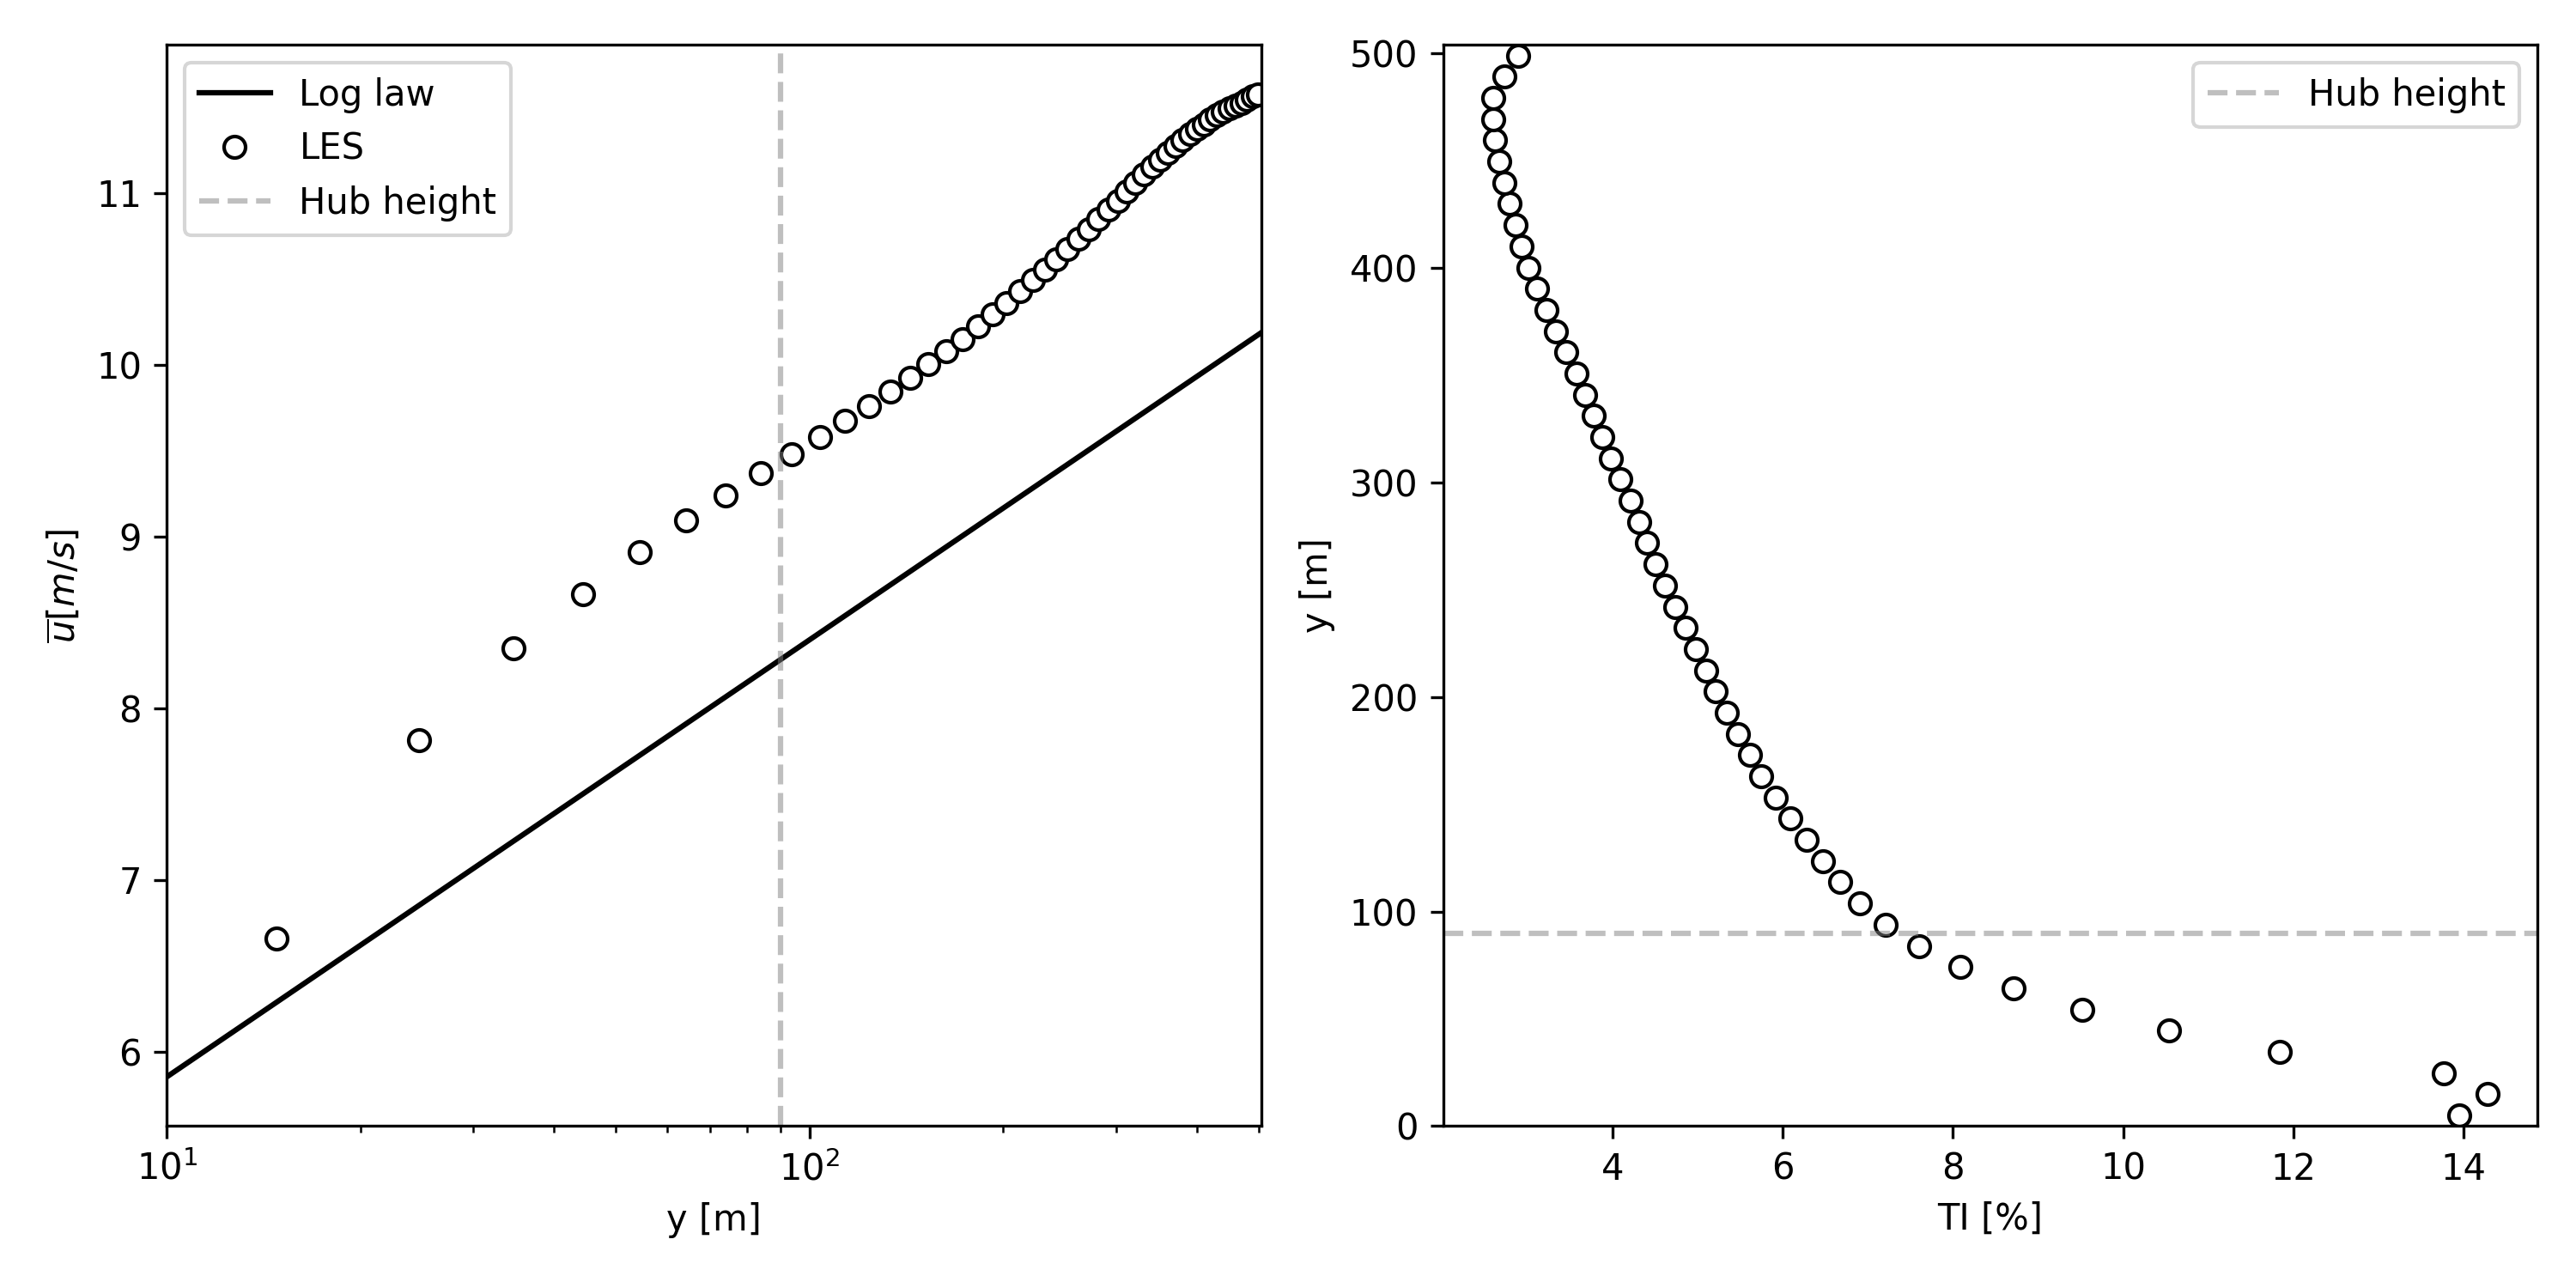
\includegraphics[scale=0.5]{precursor_stats.png}
    \caption{Mean streamwise velocity (left) and turbulence intensity (right)
    of the simulated atmospheric boundary layer}
    \label{fig:abl}
\end{figure}

The large eddy simulations were run for a $30$ minute spinup period, and power
output was averaged over a subsequent 2 hour period. Figure
\ref{fig:power_convergence} displays the trajectory of the simulated power
output over this two hour period, showing that the cumulative average power
output stabilizes relatively quickly, between 30 and 60 minutes after spinup.
This suggests that we may see significant efficiency gains from an adaptive approach
wherein the simulation duration is varied by the optimization campaign.

\begin{figure}[htbp]
    \centering
    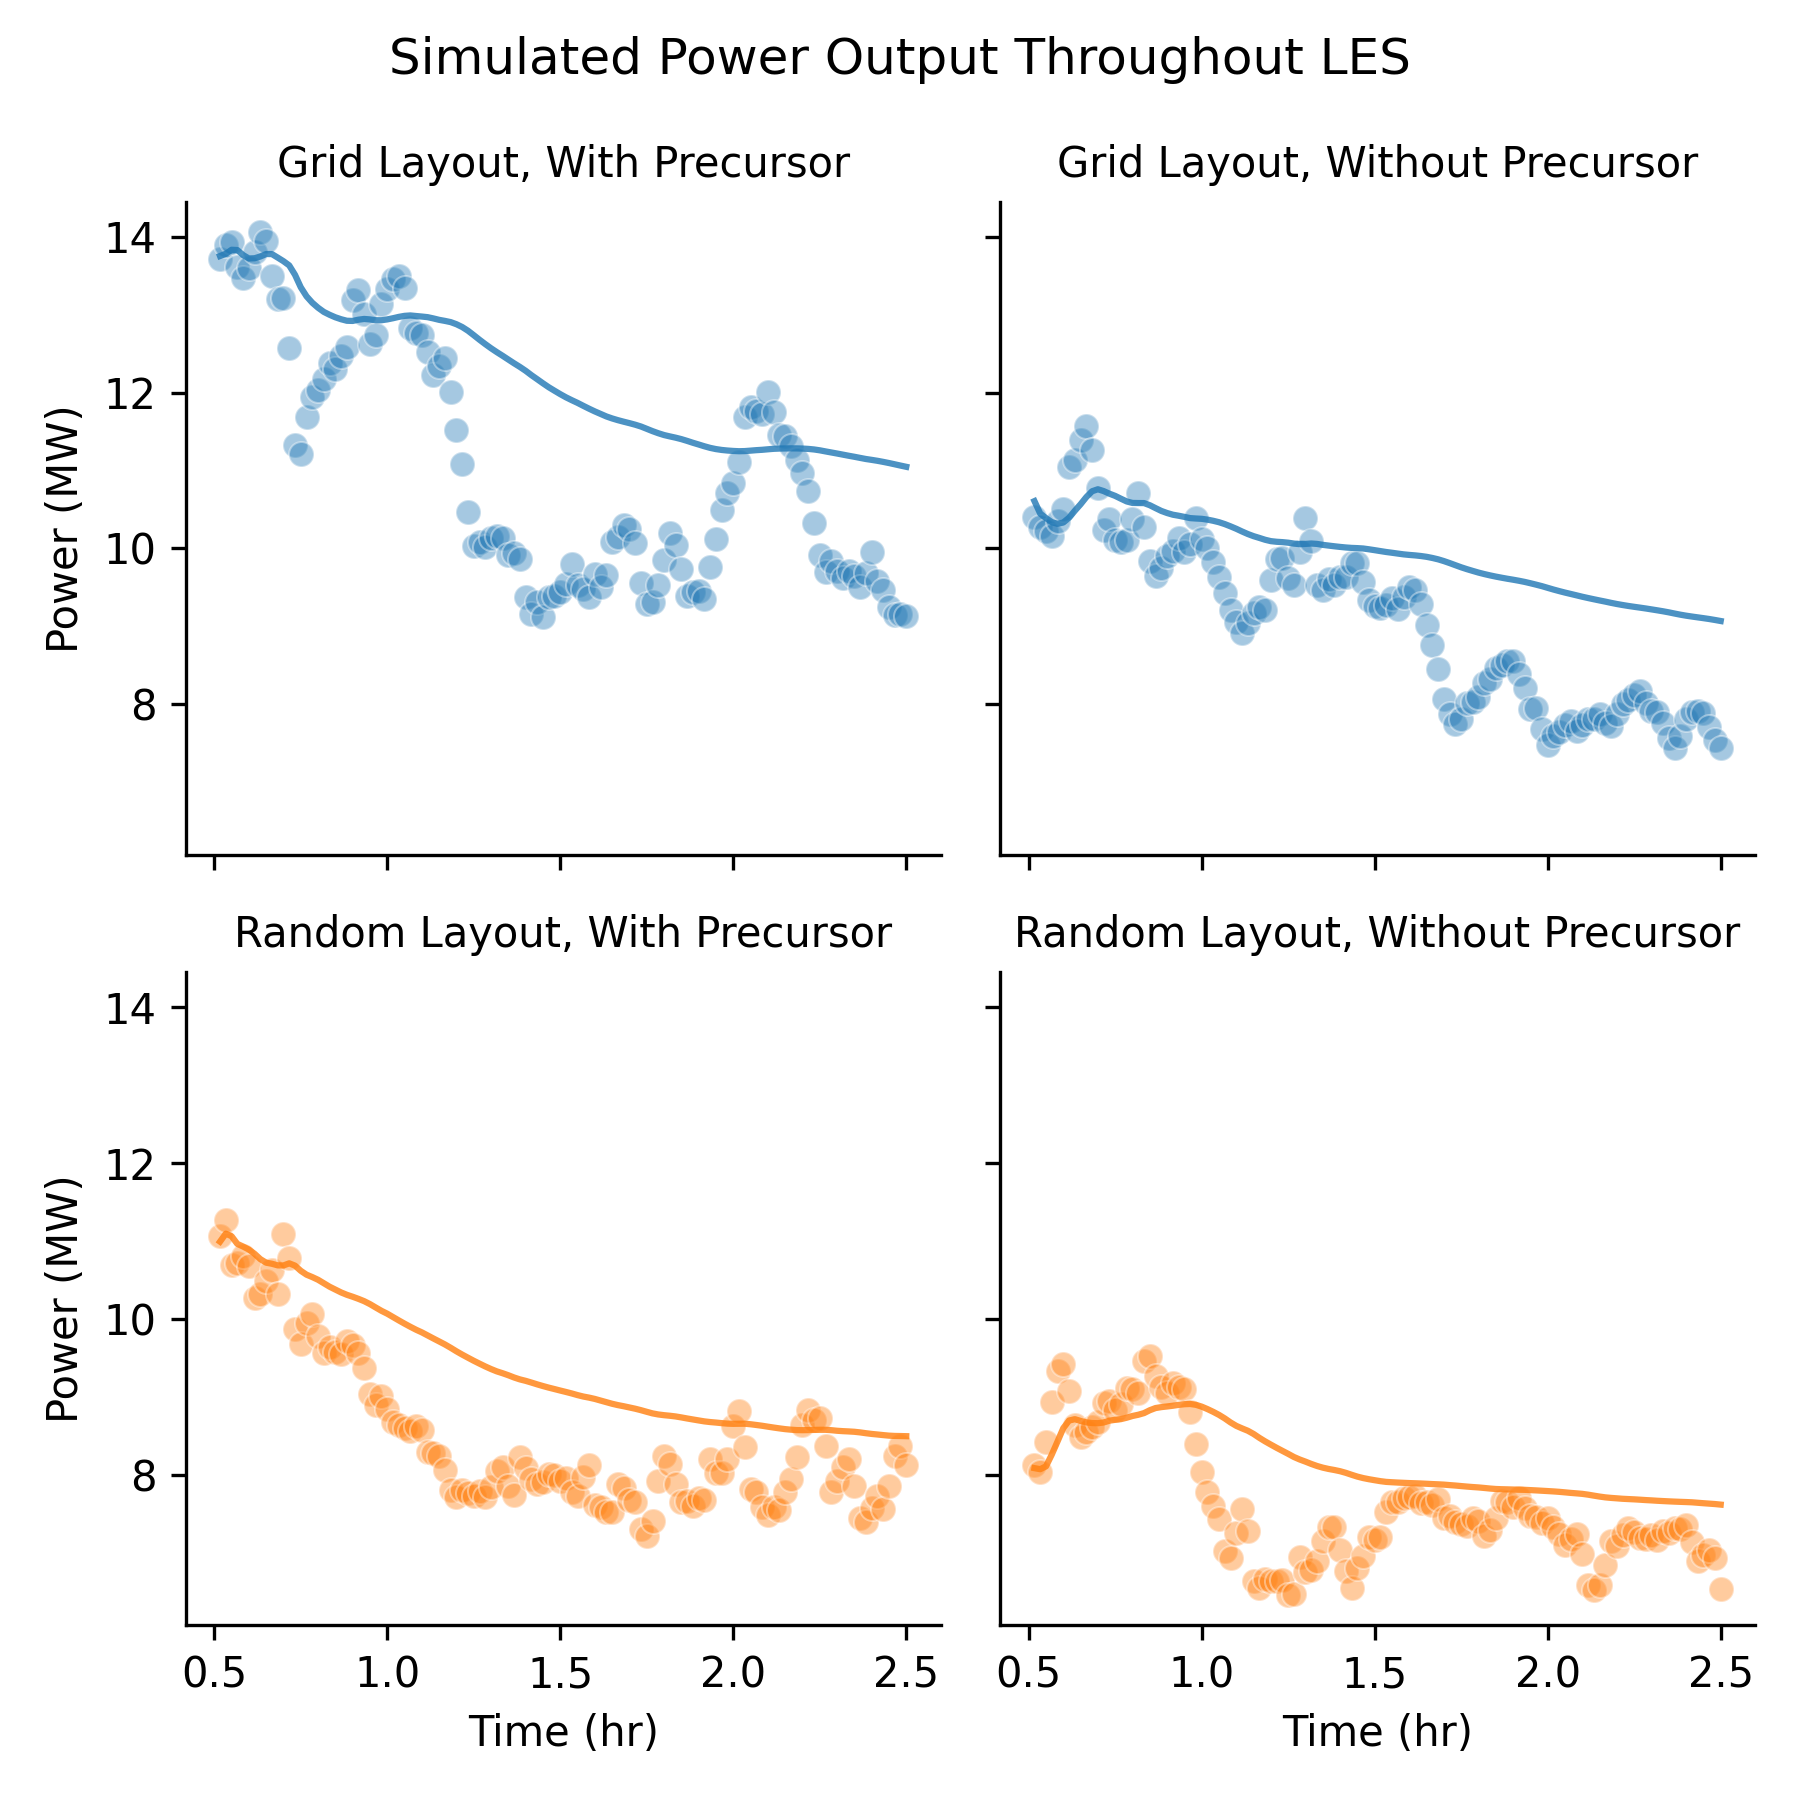
\includegraphics[scale=0.4]{power_convergence.png}
    \caption{
    Statistical convergence of simulated wind farm power output in both a grid
    and random turbine layout. All measurements were taken after a
    30 minute spinup period.
    }
    \label{fig:power_convergence}
\end{figure}


\subsection{Layout Optimization}

To allow for the kernel hyperparameters to be fit, we initialize the
optimization routine with $K_\text{approx} = 100$ prefixed evaluations from the
GCH approximation model, and $K_\text{LES} = 12$ from the large-eddy
simulation, following \cite{moleMultiFidelityBayesianOptimisation2024}. The
initial layouts were sampled using Latin hypercube sampling, along with an
additional default layout of the turbines placed in an evenly spaced grid.
Figure \ref{fig:streamwise_velocity} displays mean and instantaneous velocity simulations
for the grid layout.

\begin{figure}[htbp]
    \centering
    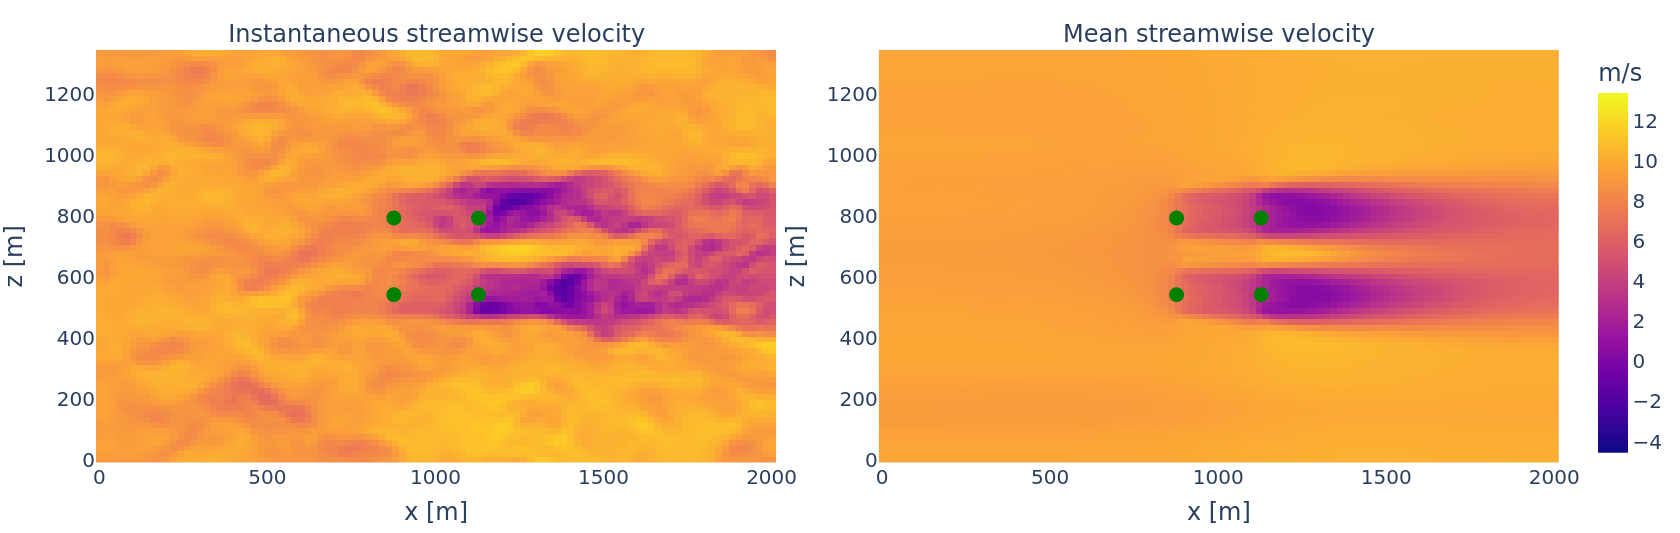
\includegraphics[scale=0.28]{grid_velocity_flow.png}
    \caption{
        Instantaneous (left) and mean (right) streamwise velocity field for a
        grid farm layout, with wind flowing in the positive x direction. The
        instantaneous field was saved 1 hour after the 30 minute spinup period.
    }
    \label{fig:streamwise_velocity}
\end{figure}

\subsection{Single-Fidelity Layout Optimization with LES}

As a baseline for comparison for the multi-fidelity layout optimization run, we
performed a single-fidelity BO campaign with large eddy simulation evalutions
only. To increase throughput and reduce the wall-clock time of each run, batch
optimization was performed, with $B = 5$ simulations run in parallel at each
optimization step. The procedure was run for 48 hours, resulting in 56 completed batches.

Figure \ref{fig:les_only_power_trajectory} displays the optimization history of
this LES-only run. The best performing layout the optimization routine identifies
achieves a power production of $14.9$ MW.

\begin{figure}[htbp]
    \centering
    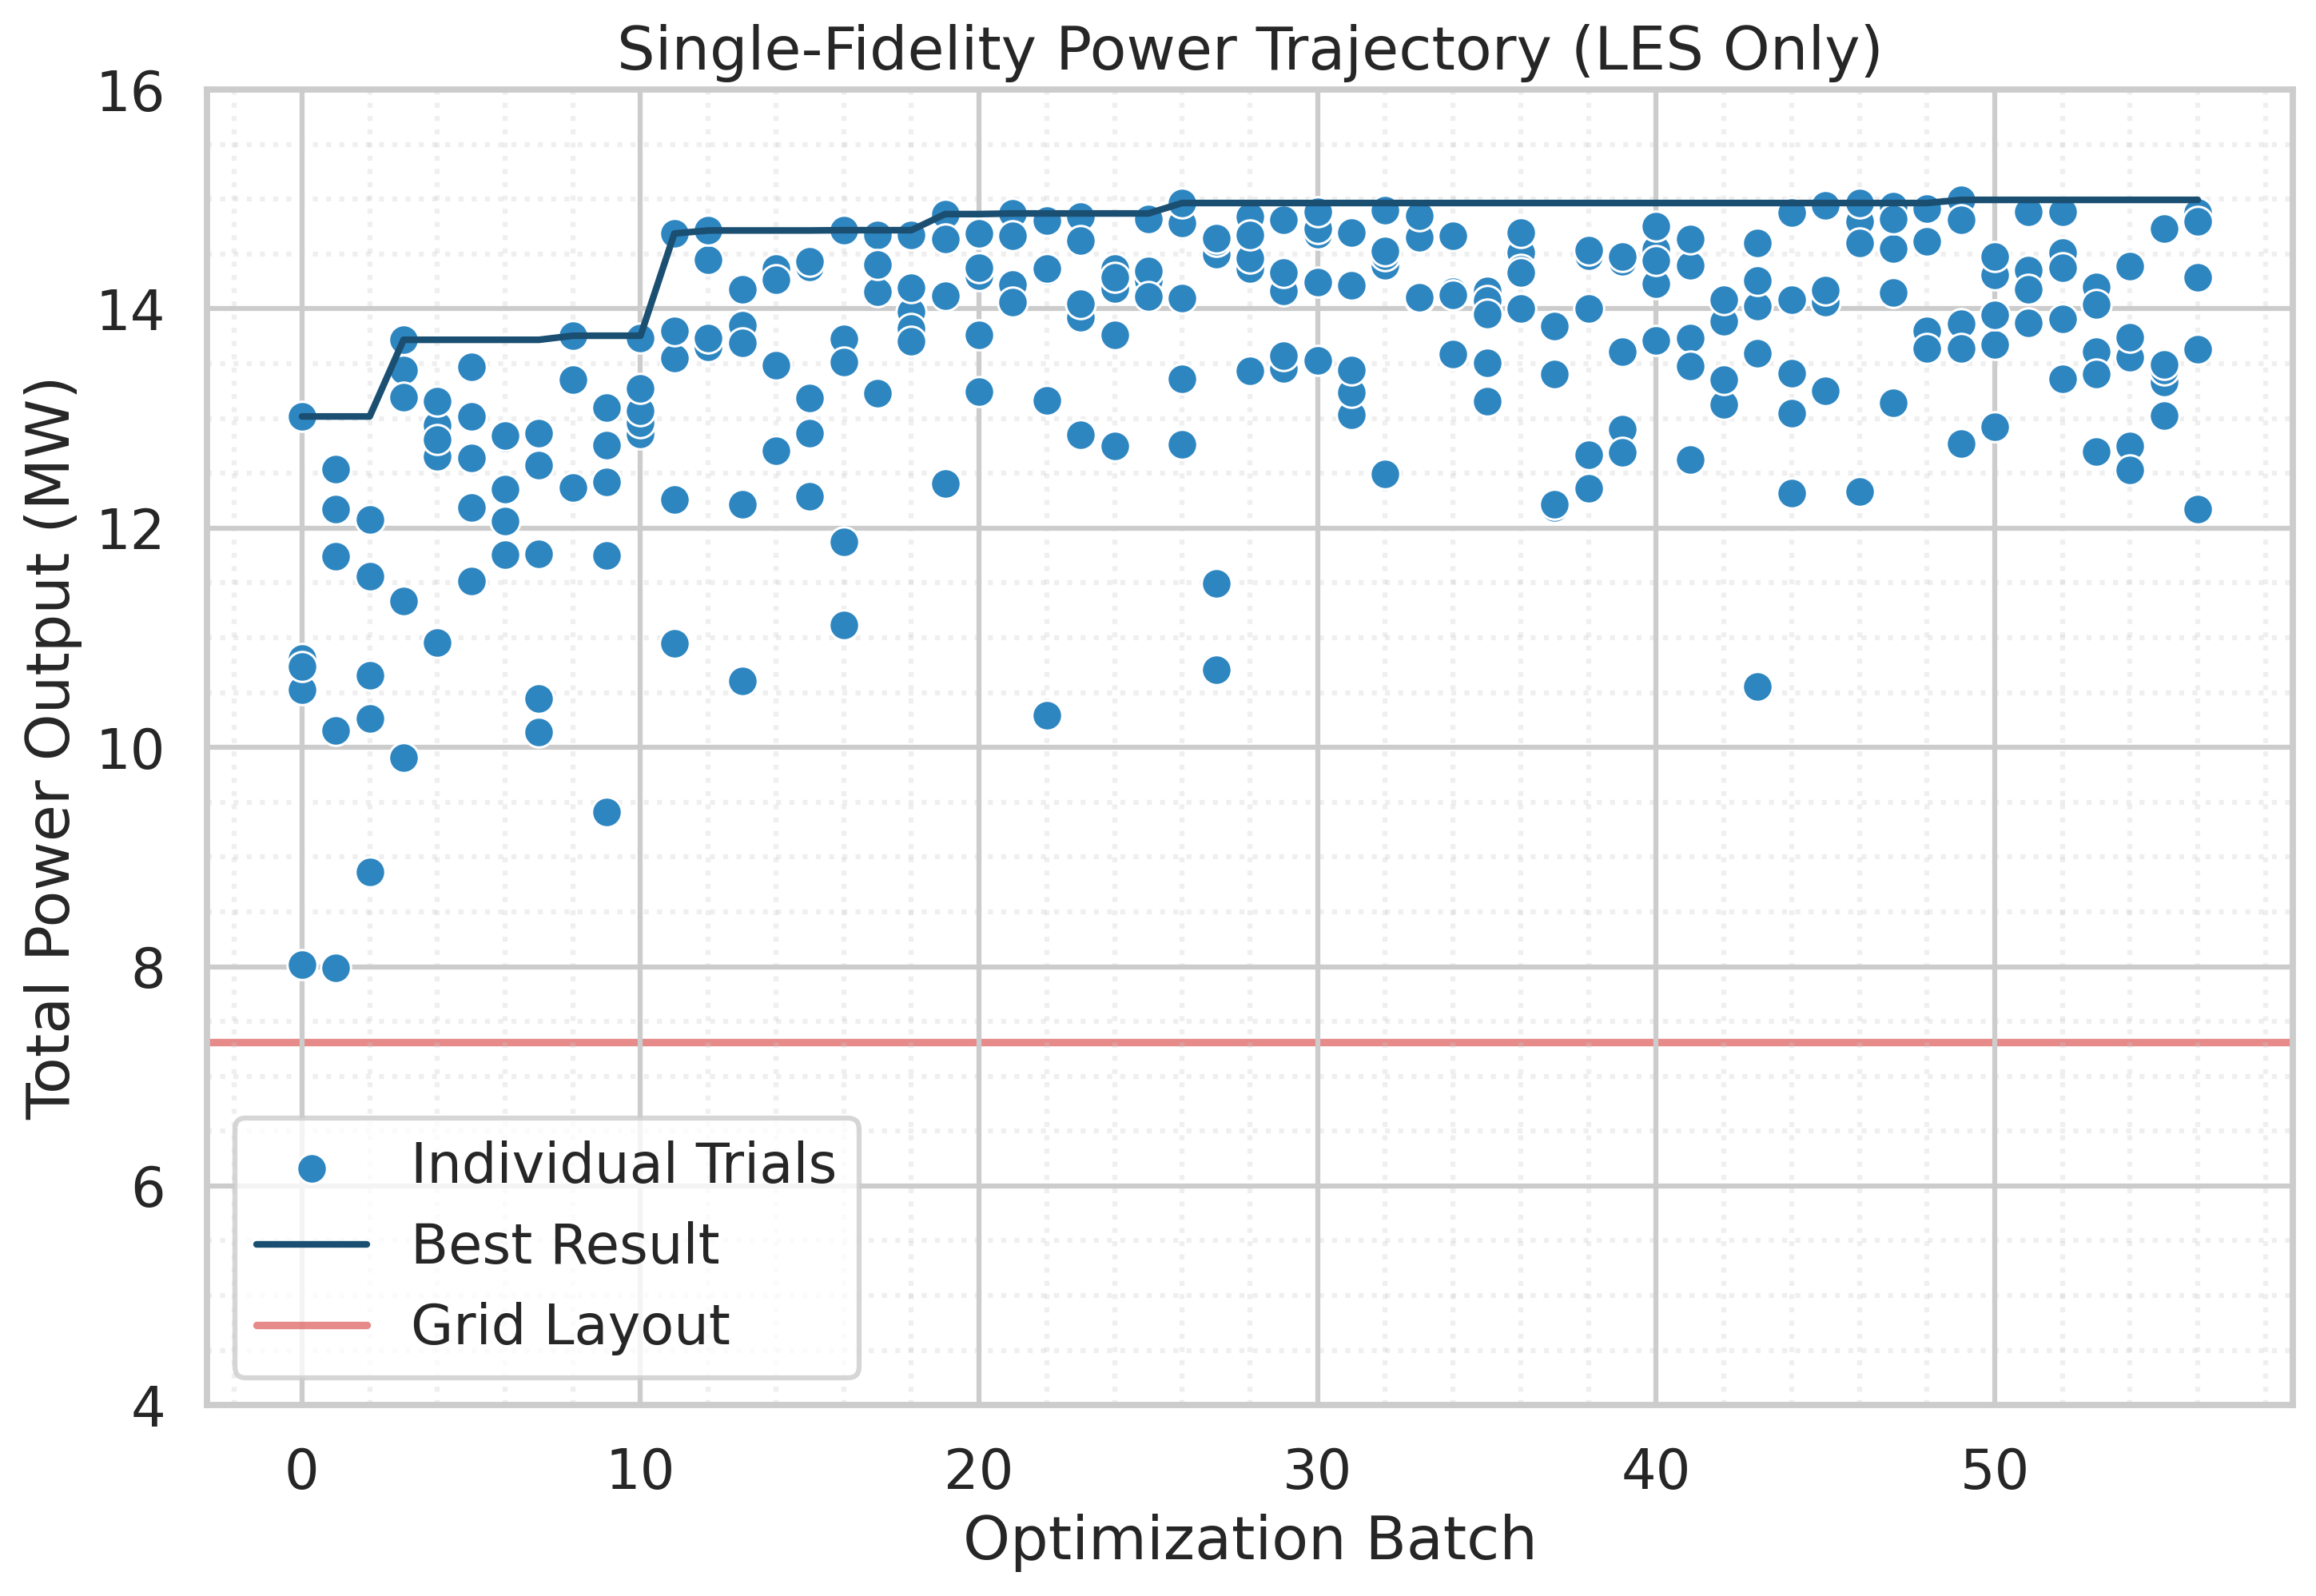
\includegraphics[scale=0.5]{../campaigns/les_only/power_trajectory.png}
    \caption{Wind farm configuration power output throughout single-fidelity
    (LES only) Bayesian layout optimization. For reference, the power
    production of a standard grid wind farm layout is displayed in red.
    }
    \label{fig:les_only_power_trajectory}
\end{figure}

\subsection{Multi-Fidelity Layout Optimization}
The multi-fidelity layout optimization run was performed by alternating
evaluation batches between GCH and LES observations, as described in Section
\ref{sec:opt_approach}. At each step, we employed batch sizes of $B_\text{GCH}
= 50$ and $B_\text{LES} = 4$. The power trajectory for this optimization run is
also displayed in Figure \ref{fig:multi_fidelity_power_trajectory}.

Again, this layout optimization procedure was allowed 24 hours to run. It was
able to complete 21 full evaluation rounds, totaling 525 GCH evaluations and 84
LES evaluations. 

The best layout found by the multi-fidelity campaign is slightly worse than
the best found by the single-fidelity campaign, at 14.6 MW.

The multi-fidelity campaign is able to find a near-final layout
achieving 14.5 MW within the first 4 large eddy simulation batches. By contrast,
the single-fidelity campaign does not find a configuration producing more than 14 MW
until the 12th batch. As expected, having access to the GCH evaluation fidelity
significantly speeds up optimization progression. This result raises the interesting question
of how the performance difference might change under a more difficult layout optimization
problem with more turbines, a regime where sample efficiency may be far more important.

\begin{figure}[htbp]
    \centering
    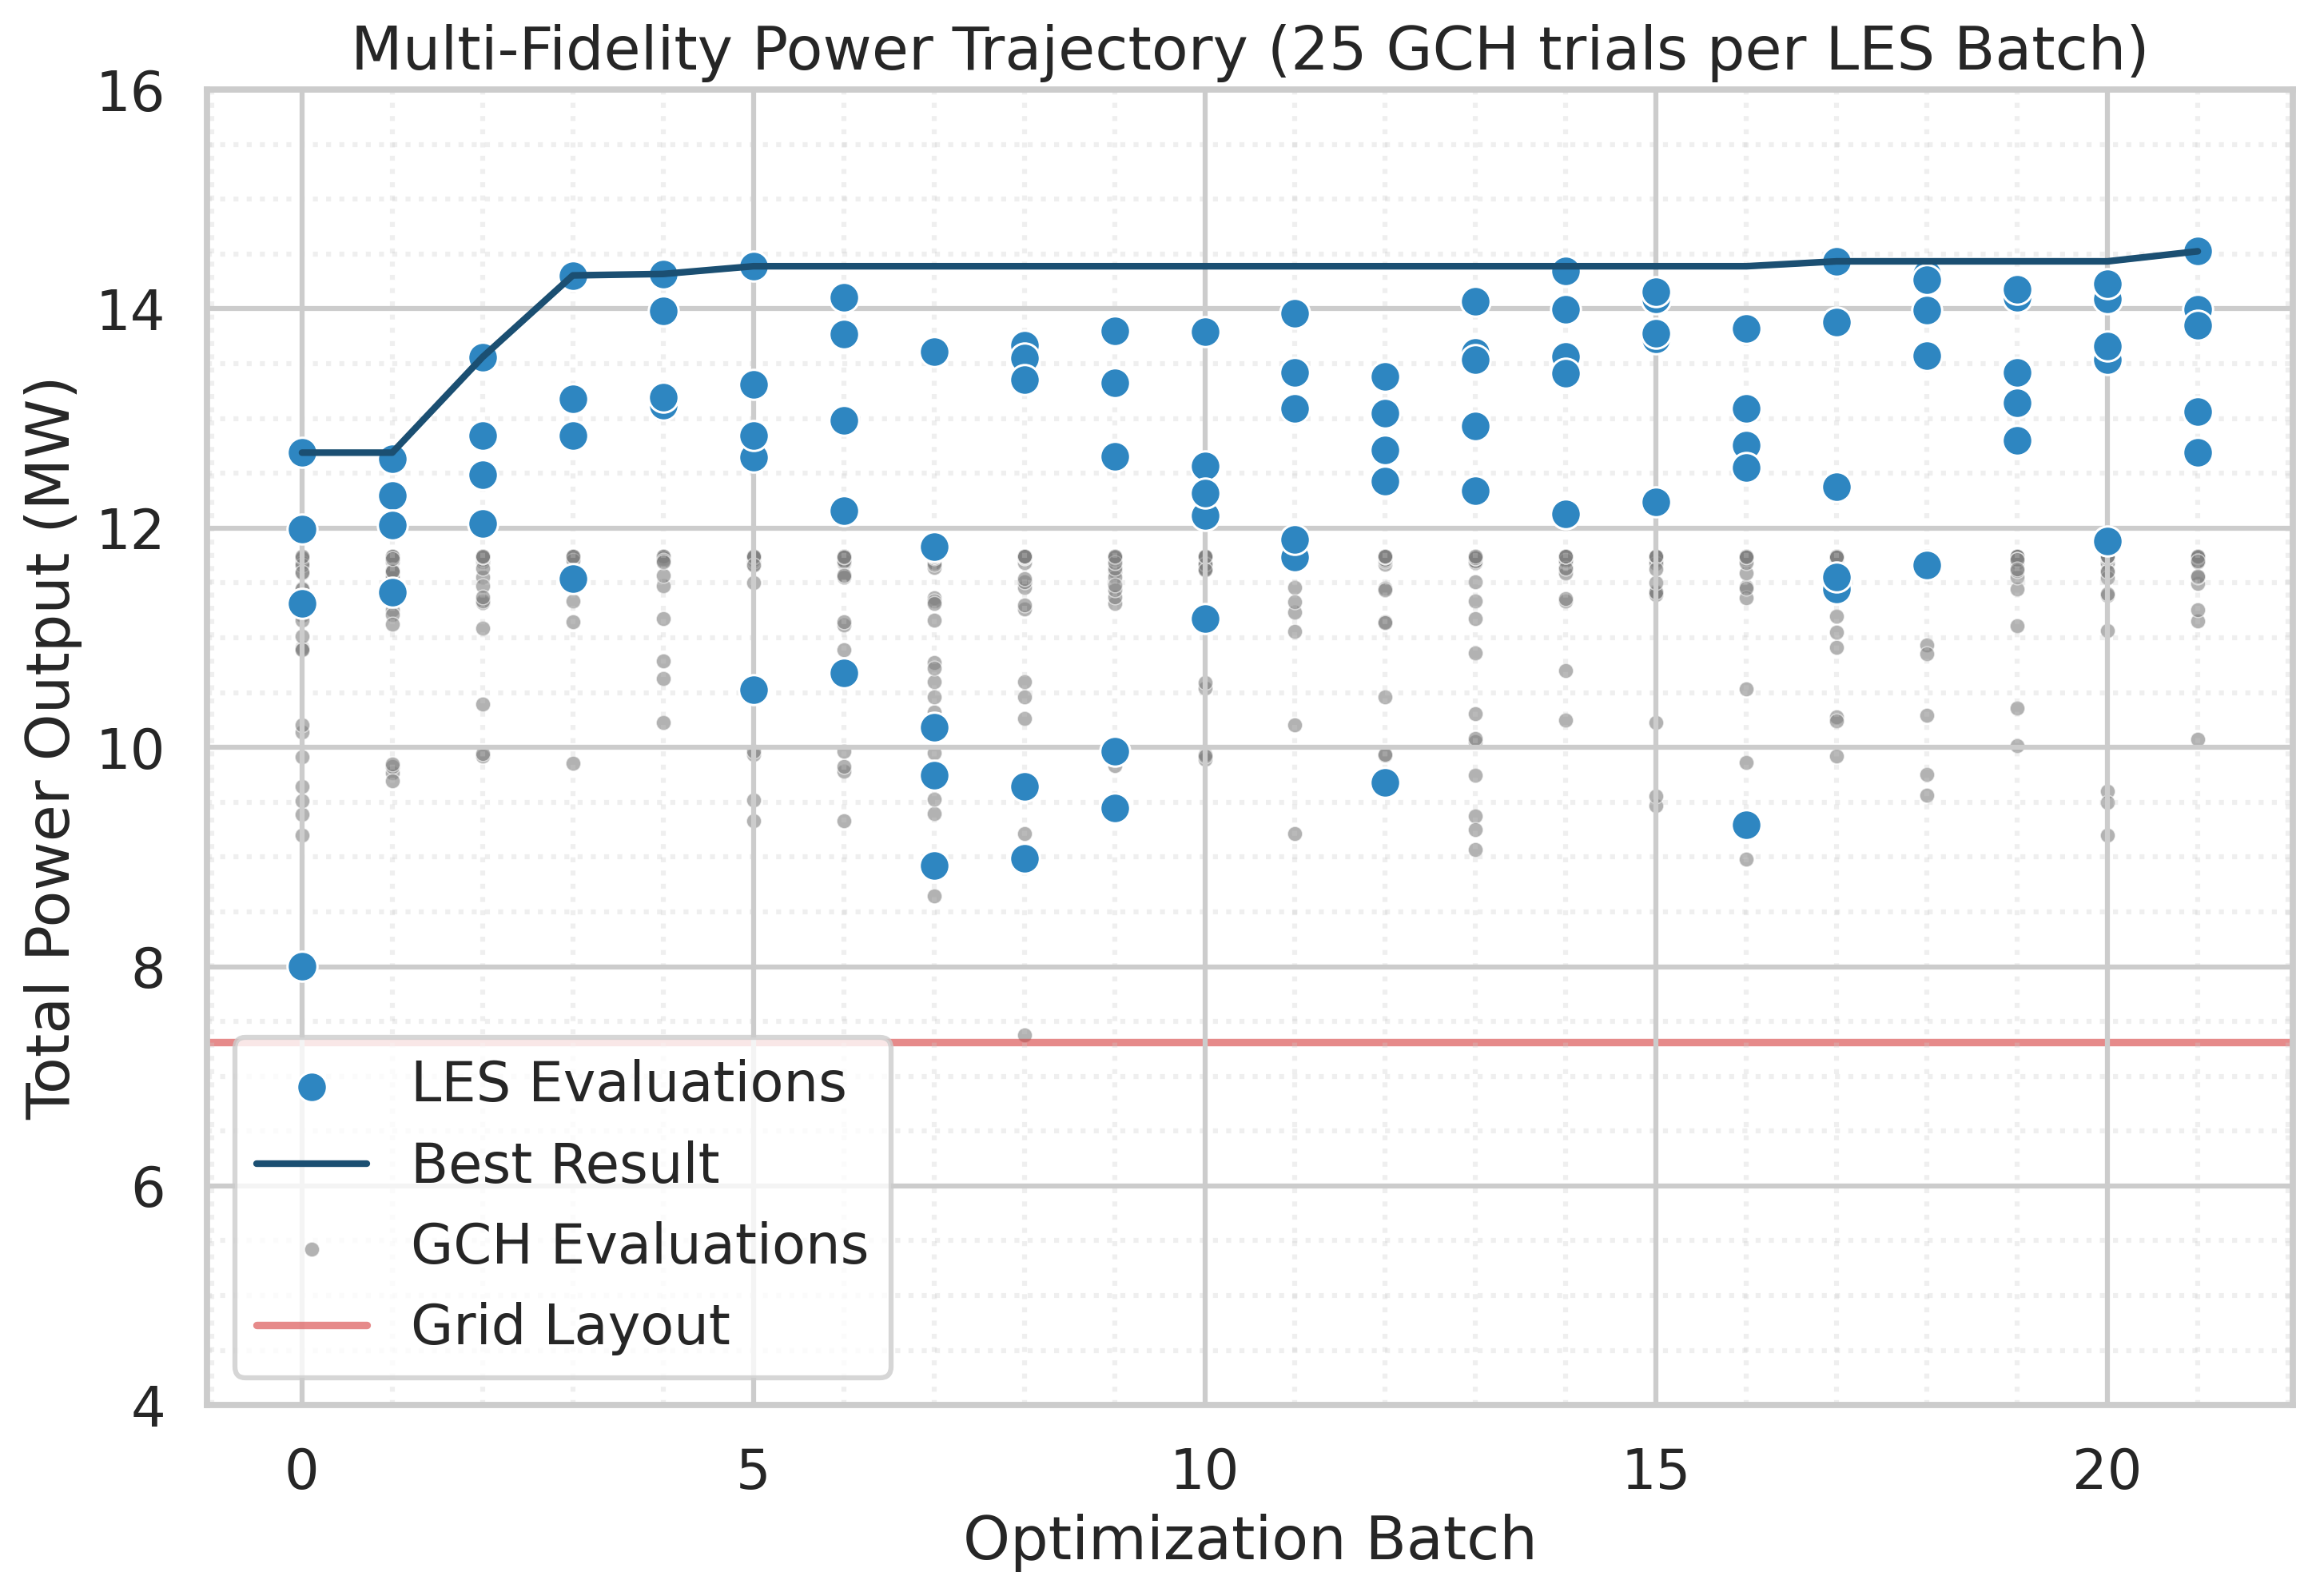
\includegraphics[scale=0.5]{../campaigns/mf_alternating/power_trajectory.png}
    \caption{Wind farm configuration power output throughout multi-fidelity
    Bayesian layout optimization. Low-fidelity approximate evaluations using
    GCH are shown in grey, and expensive high-fidelity LES evaluations are shown in blue.
    For reference, the power production of a standard grid wind farm layout is
    displayed in red.
    }
    \label{fig:multi_fidelity_power_trajectory}
\end{figure}

\section{Discussion}
This work demonstrates the potential benefits of multi-fidelity Bayesian
optimization for wind farm layout optimization, while also highlighting several
promising directions for future research.

First, our results suggest that multi-fidelity optimization can achieve
near-optimal layouts with significantly fewer expensive LES evaluations
compared to single-fidelity approaches. However, the current study's limitation
to just four turbines leaves open the question of how these benefits scale to
more realistic wind farm configurations. We hypothesize that the sample
efficiency gains from multi-fidelity optimization will become even more
pronounced as the dimensionality of the layout optimization problem increases.

Several methodological extensions could significantly improve the practical
utility of this approach:

\begin{enumerate}
    \item \textbf{Adaptive Fidelity Selection:} Rather than manually
        alternating between GCH and LES evaluations, implementing cost-aware
        acquisition functions (like that of \cite{wuPracticalMultifidelityBayesian2019}) could
        automatically balance the exploration-exploitation trade-off across
        fidelities.     
    \item \textbf{Variable Wind Conditions:} The current work considers only a
        single inflow wind direction and speed. Extending the optimization to handle
        varying inflowing wind speeds and directions would better reflect real-world conditions.
    
    \item \textbf{Adaptive LES Duration:} Our convergence analysis (Figure
        \ref{fig:power_convergence}) suggests that power output statistics
        stabilize relatively quickly. This opens the possibility of adaptively
        selecting simulation durations, potentially reducing computational cost
        without sacrificing accuracy. Early optimization iterations might use
        shorter simulations, with longer durations reserved for promising
        configurations.

    \item \textbf{Grey-box Optimization:} Currently, we treat each LES
        evaluation as a black box, only observing the final time-averaged power
        output. However, the LES solver produces rich intermediate results
        throughout its run, including instantaneous power measurements and
        velocity field data. A grey-box Bayesian optimization approach could
        leverage these intermediate observations to make early stopping
        decisions or guide the selection of subsequent layouts, potentially
        yielding significant efficiency improvements.
\end{enumerate}

\section{Code Availability}
The implementation of the methods described in this paper, including
optimization routines and simulation configurations, is available at
\href{https://github.com/amanchoudhri/windopt}{https://github.com/amanchoudhri/windopt}.

\section{Acknowledgements}
Major thanks to Prof. Nikos Bempedelis of Queen Mary University of London for
his detailed guidance on large eddy simulation configuration and BO approaches
to the layout optimization problem. A further thanks to Prof. John Cunningham
of Columbia for his instruction on Bayesian Optimization during Columbia's STAT6103 Applied Statistics
course, and his help on the framing of this paper and shaping the
future directions of the methods explored.

\newpage

\printbibliography

\newpage

\appendix 

\counterwithin{figure}{section}
\counterwithin{table}{section}

\section{Large-Eddy Simulations}

\subsection{Configuration and Parameters}

The classic Smagorinsky subgrid scale model was used, with the Smagorinsky
constant taken as $\kappa = 0.14$. Wall damping was used according to the
Mason and Thomson formulation \cite{masonStochasticBackscatterLargeeddy1992},
with a damping growth parameter of $n = 3$.

The forward timesteps were calculated using a third-order Runge-Kutta scheme.
Simulations were run with inflow/outflow boundary conditions in the streamwise
direction, periodic conditions in the spanwiise direction, and free-slip
conditions in the vertical direction.

The actuator disks were modeled using the following common parameters:

\begin{table}[h]
    \centering
    \caption{Actuator Disk Parameters}

    \vspace{0.75em}

    \begin{tabular}{c|c}
        Parameter & Value \\
        \hline
        Axial induction factor, $a$ & 0.25 \\
        Thrust coefficient, $C_T$ & 0.75
    \end{tabular}

\end{table}

\subsection{Precursor Simulations}

The precursor simulation was run for a total of $72,000$ timesteps, or 4 hours. Outflow
velocity planes were collected and saved following a 2 hour (7200 timestep) spinup period.

A moderate deviation from the log law profile expected under a simulation of a
neutral ABL is observed in Figure \ref{fig:abl}. This deviation is likely due
to the horizontal resolution of the computational mesh used in the precursor
simulation, at $\Delta x \approx \Delta z \approx 20m$. Figures \ref{fig:supp_abl_40m}
and \ref{fig:supp_abl_10m} illustrate this point,
displaying profiles for ABLs simulated under other horizontal mesh resolutions.

\begin{figure}[ht]
    \centering
    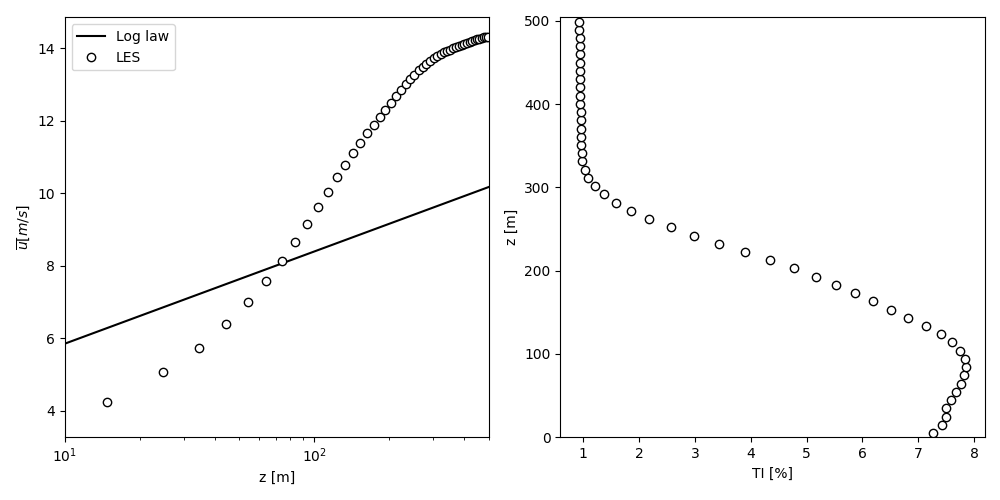
\includegraphics[scale=0.5]{40m_precursor_stats.png}
    \caption{Precursor ABL Profile for Coarser Horizontal Mesh Resolution, $\Delta x = \Delta z = 40m$}
    \label{fig:supp_abl_40m}
\end{figure}

\begin{figure}[ht]
    \centering
    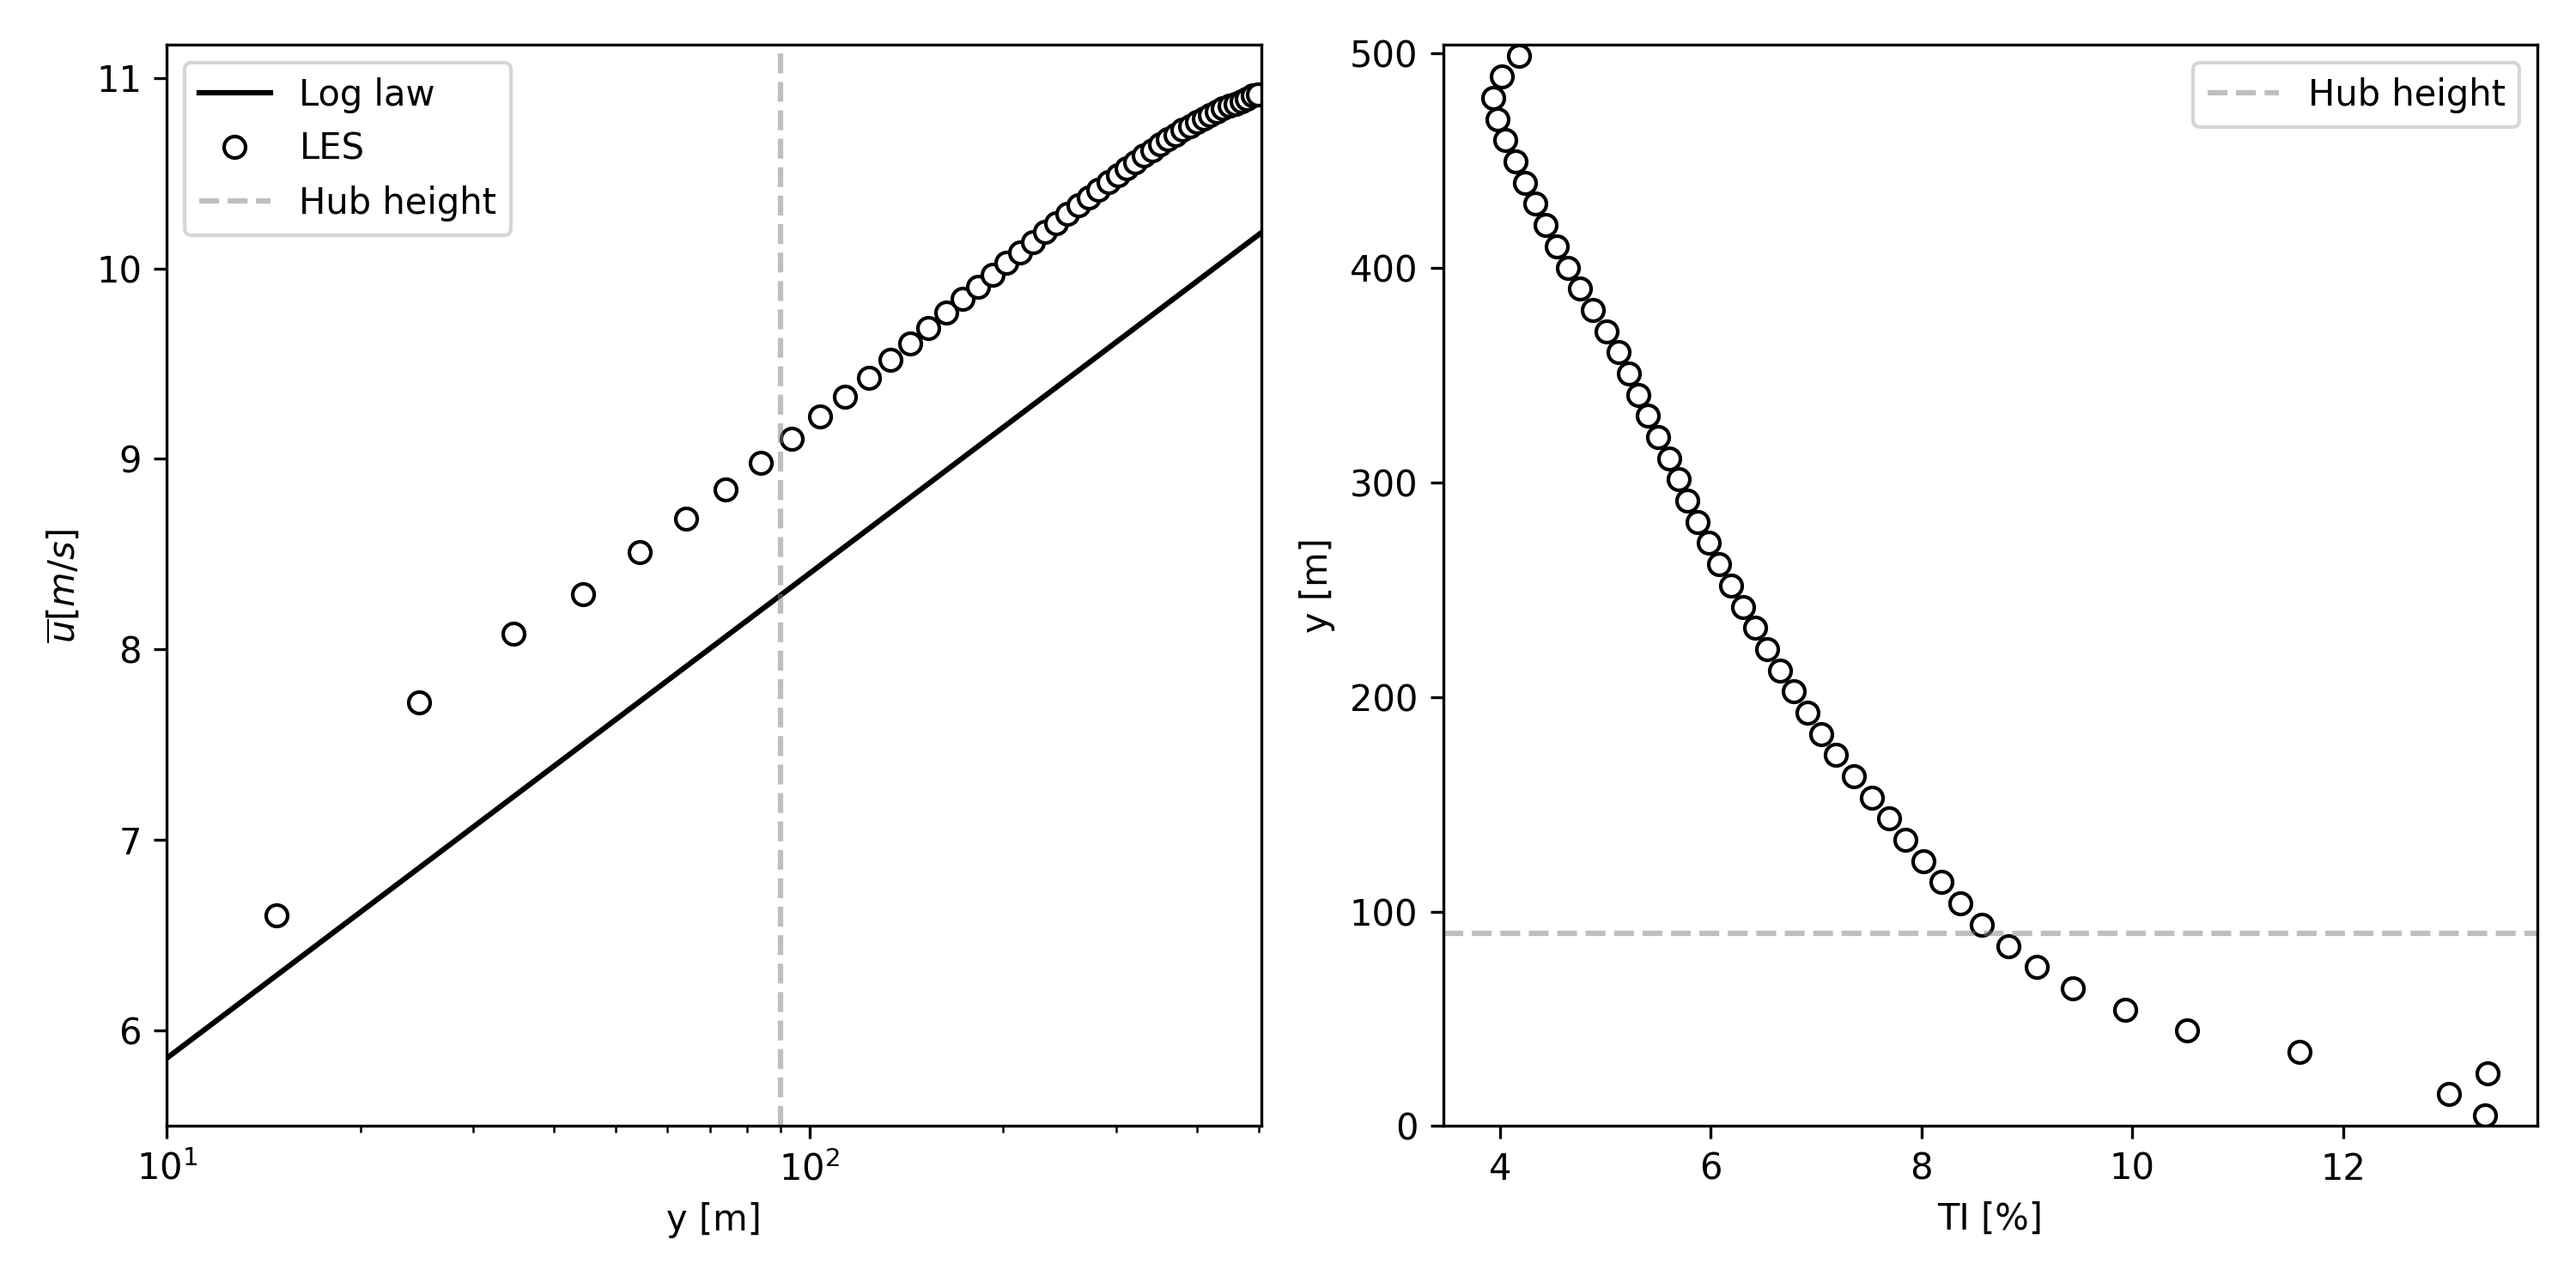
\includegraphics[scale=0.5]{10m_precursor_stats.png}
    \caption{Precursor ABL Profile for Finer Horizontal Mesh Resolution, $\Delta x = \Delta z = 10m$}
    \label{fig:supp_abl_10m}
\end{figure}

\section{Computational Details}
Large-eddy simulations were computed via parallelization across 8 nodes of
Columbia's Terremoto cluster. Each node has two 12-core CPUs, for a total of
192 cores involved in computing each simulation. The CPUs used were Intel Xeon
Gold 6127 2.6 GHz processors.

Under this configuration, the scaling time of the large-eddy simulations
was roughly 2.5 simulated wind farm seconds per wall-clock second.
\end{document}

%%% Local Variables:
%%% mode: latex
%%% TeX-master: t
%%% End:
% fonts
